% vim:autoindent:set textwidth=78:

\section{Come iniziare}\label{label_getstarted}

% when the revision of a section has been finalized, 
% comment out the following line:
% \updatedisclaimer

Questo capitolo fornisce una veloce panoramica dell'installazione
di QGIS, alcuni dati campione dall'homepage di QGIS e su come avviare
una prima semplice sessione in cui vengano visualizzati layer raster
e vettoriali.

\subsection{Installazione}\label{label_installation}
\index{installation}

L'installazione di QGIS è molto semplice. Pacchetti standard per l'installazione
sono disponibili per MS Windows e Mac OS X. Per le distribuzioni GNU/Linux
sono disponibili pacchetti binari (rpm and deb) o repositories software
da aggiungere al gestore di installazione. Informazioni aggiornate
possono essere reperite sul sito web di QGIS \url{http://qgis.osgeo.org/download/}.

La compilazione di QGIS da sorgenti è documentata nell'Appendice \ref{sec:install_windows}
per MS Windows \win, Appendice \ref{sec:install_macosx} per Mac
OSX \osx e Appendice \ref{sec:install_linux} per GNU/Linux \nix.
Le istruzioni per l'installazione sono distribuite con il codice sorgente
di QGIS e sono anche disponibili su \url{http://qgis.osgeo.org}.

\subsection{Dati campione}\label{label_sampledata}
\index{data!sample} 

La guida utente contiene esempi basati sul set di dati campione di
QGIS.

\win L'installer per Windows comprende un'opzione per scaricare il
set di dati campione di QGIS. Se selezionato, i dati verranno scaricati
nella vostra cartella \filename{My Documents} e posizionata in
una cartella denominata \filename{GIS Database}. Può essere usato
Windows Explorer per spostare in questa cartella in qualunque altra
posizione. Qualora non fosse stata selezionata l'opzione di installare
il set di dati campione durante l'installazione iniziale di QGIS è
possibile: 
\begin{itemize}
\item usare dati GIS già posseduti; 
\item scaricare il set di dati dal sito di QGIS \url{http://qgis.osgeo.org/download};
oppure 
\item disinstallare QGIS e reinstallarlo selezionando l'opzione per lo scaricamento
dei dati. 
\end{itemize}

\nix \osx Per GNU/Linux e Mac OSX non sono ancora disponibili pacchetti
di installazione del set di dati campione in formato rpm, deb or dmg.
Per usare il set di dati campione scaricate il file \filename{qgis\_sample\_data}
come archivio ZIP o TAR da \url{http://download.osgeo.org/qgis/data/}
e decomprimetelo sul vostro sistema. Il dataset Alaska include tutti
i dati GIS che sono usati come esempi e schermate nella guida utente,
e inculde anche un piccolo database GRASS. La proiezione usata per
il set di dati di QGIS è Alaska Albers Equal Area con unità in piedi.
Il codice EPSG di questa proiezione è 2964.

\begin{verbatim}
PROJCS["Albers Equal Area",
    GEOGCS["NAD27",
        DATUM["North_American_Datum_1927",
            SPHEROID["Clarke 1866",6378206.4,294.978698213898,
                AUTHORITY["EPSG","7008"]],
            TOWGS84[-3,142,183,0,0,0,0],
            AUTHORITY["EPSG","6267"]],
        PRIMEM["Greenwich",0,
            AUTHORITY["EPSG","8901"]],
        UNIT["degree",0.0174532925199433,
            AUTHORITY["EPSG","9108"]],
        AUTHORITY["EPSG","4267"]],
    PROJECTION["Albers_Conic_Equal_Area"],
    PARAMETER["standard_parallel_1",55],
    PARAMETER["standard_parallel_2",65],
    PARAMETER["latitude_of_center",50],
    PARAMETER["longitude_of_center",-154],
    PARAMETER["false_easting",0],
    PARAMETER["false_northing",0],
    UNIT["us_survey_feet",0.3048006096012192]]
\end{verbatim}

Se si intende usare QGIS come frontend a GRASS, delle "locations" campione
(ad es. Spearfish or South Dakota) sono disponibili sul sito ufficiale
di GRASS GIS \url{http://grass.osgeo.org/download/data.php}.

\subsection{Sessione di esempio}\label{samplesession}

Ora che si è installato QGIS e si ha a disposizione un set di dati
campione, dimostreremo una breve e semplice sessione di QGIS. Visualizzeremo
un layer raster ed uno vettoriale. Useremo il layer raster dell'uso
del suolo \filename{qgis\_sample\_data/raster/landcover.img} e
il layer vettoriale dei laghi \filename{qgis\_sample\_data/gml/lakes.gml}.

\minisec{Avvio di QGIS}

\begin{itemize}
\item \nix {Avviate QGIS scrivendo: \usertext{qgis} al prompt dei comandi.} 
\item \win {Avviate QGIS usando il menu Start o l'icona sul desktop, oppure
facendo doppo click su un file di progetto QGIS.} 
\item \osx {Doppio click sull'icona nella cartella Applicazioni.}
\end{itemize} 

\minisec{Caricare dati raster e vettoriali dal set di dati campione}

\begin{enumerate}
\item Cliccate sull'icona \toolbtntwo{mActionAddRasterLayer}{Carica layer raster}. 
\item Individuate la cartella \filename{qgis\_sample\_data/raster/},
selezionate il file ERDAS Img \filename{landcover.img} e cliccate
\button{Apri}. 
\item Ora cliccate sull'icona \toolbtntwo{mActionAddOgrLayer}{Carica layer vettoriale}. 
\item Individuate la cartella \filename{qgis\_sample\_data/gml/}, selezionate
il file GML \filename{lakes.gml} e cliccate \button{Apri}. 
\item Ingrandite un pò la visuale su un'area a vostra scelta con alcuni laghi. 
\item Fate doppio click sul layer \filename{lakes} nella legenda per
aprire la finestra \dialog{Proprietà del layer}. 
\item Cliccate sulla linguetta \tab{Simbologia} e selezionate blu come
colore di riempimento. 
\item Cliccate sulla linguetta \tab{Etichette} e spuntate l'opzione \checkbox{Mostra
etichette} per abilitare l'etichettatura. 
\item Cliccate \button{Applica}.
\end{enumerate} 

\begin{figure}[ht]
   \begin{center}
   \caption{Una sessione di esempio in QGIS \nixcaption}\label{fig:simple_session}\smallskip
   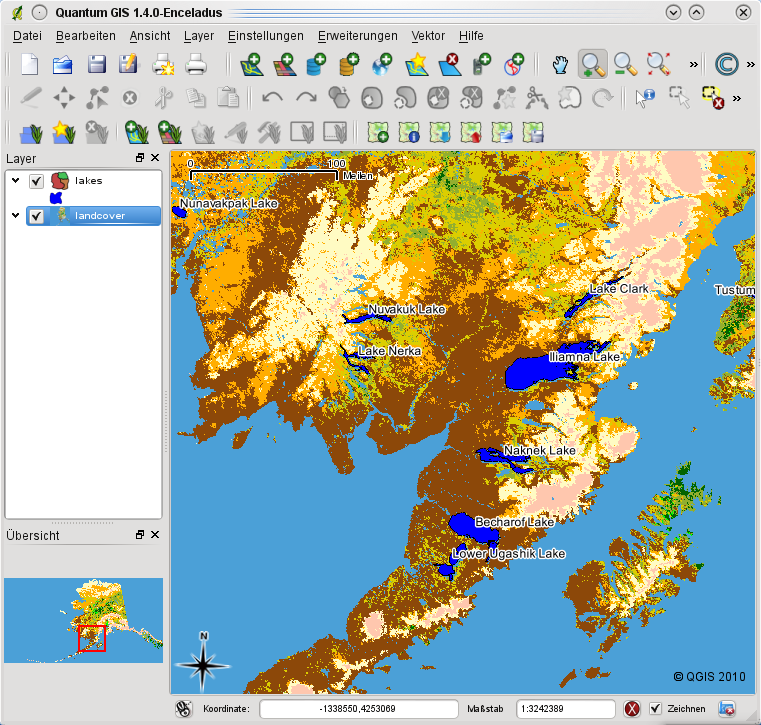
\includegraphics[clip=true, width=14cm]{simple_session}
\end{center}  
\end{figure}

Visto come è facile visualizzare layer raster e vettoriali in QGIS?
Proseguiamo alla sezione seguente per imparare ulteriori funzioni
disponibili, caratteristiche e settaggi e come usarle.
